\subsection{Answers}
\subsubsection{Is the project alive?}
We are going to use \textbf{time} as the basis to which we are going to attach the metrics, if we see an increase over time around a project we could say that a project has an active community and the contributions, which could be issues or commits, are increasing over time, otherwise, if we see a decline we can see how steep this decline is, and raise that so the contributor takes that into consideration.

\paragraph{Trend of commits over the years:} 

We use the following data set \cite{trend-of-commits-over-the-years} that count all the commits that were performed for each project each year and we plot it in the chart below.
\begin{center}
    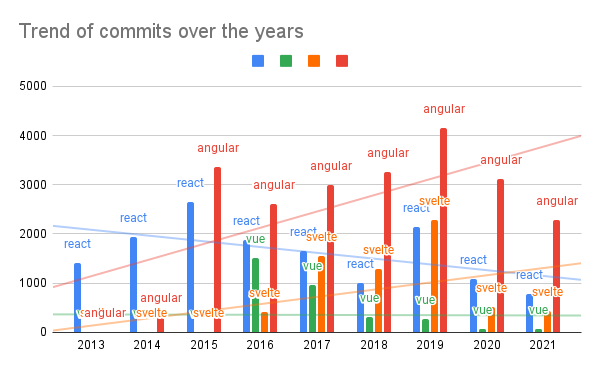
\includegraphics[scale=0.35]{trend-of-commits-over-the-years}    
\end{center}

We can see that for React an increase in the first 3 years but after that, there has been a decline in the number of commits, on the other hand, we can see that angular started one year later after react and it surpassed it in 2015, and the rate of commits has been increasing ever since.

Vue and Svelte are the newest frameworks, both conceive in 2016, Vue's contribution has been more stable over the last few years while svelte has a trend of increasing, and the amount of commits seems to surpass Vue most years.

Even though react is the only project that has a declining trendline we don't think that is dying, if we take a look at the table provided in the section \textit{Current state of the world}, react is used by 7.6 million projects.

We can't take react outside of the context in which it was born, inside Facebook, to standardize the way that developers create user interfaces, we attribute this decline to the maturity of the framework, using the Capability maturity model \cite{cmm}, tell us that the project is at level 5, and their focus right now is to improve performance while keeping the stability of the project.

\paragraph{Trend of opened issues over the years: }
The last trend tells us how developers interact with the project, while this trend emphasizes how the community interacts with the project, issues are the social component in open source, at least in GitHub.

In the following chart, we did the same approach as before, we take all the data where the issues were open and we grouped them by year, and we put the projects next to each other to get any insights, below we have a chart that depicts a summary of the issues over the years, for this we use the following data set \cite{trend-of-open-issues-over-the-years}.

\begin{center}
    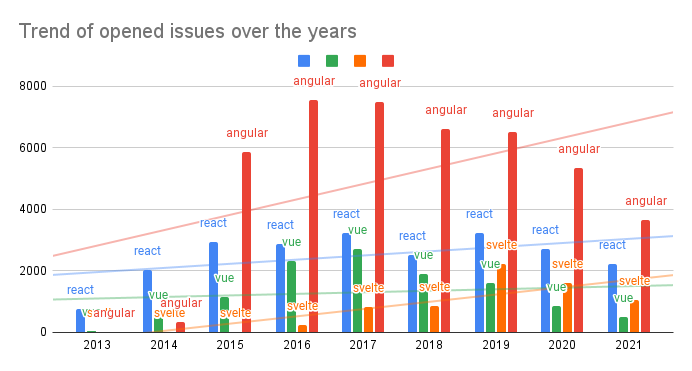
\includegraphics[scale=0.35]{trend-of-open-issues-over-the-years}    
\end{center}

From the following chart we can see that angular has the most active community overall, from react we can see that we have an increasing trendline over the years, which contrast with the decline that it's perceived from the previous trend, which helps with the assumption that we make before that commit's alone are not a single representative metric that provides \textit{liveliness} to a project, Vue has a slight increase over the years and has the same trend behavior that was displayed in the previous trend, svelte seems to have an increase trendline as well, surpassing Vue community in the last 3 years.

This could tell us that overall, all of these communities are fairly active which suggests that the project is alive, from a social aspect.

\paragraph{Trend of unique contributors per year}
We already saw the number of contributions a code received, in the form of commits, and how the community interacts with each other, now are we going to see how big the community is by the number of unique developers that contribute to the project, we are going to use the following data set\cite{trend-of-unique-contributors-per-year} to create the chart that is shown below.

\begin{center}
    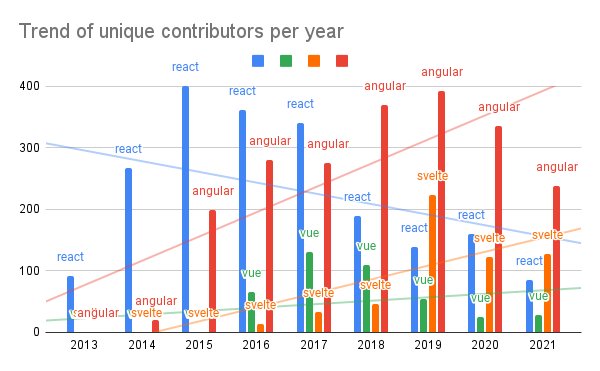
\includegraphics[scale=0.35]{trend-of-unique-contributors-per-year}    
\end{center}

From the chart we can see a decline in React from 2015 to 2021, it could be because at the beginning more developers were joining but with the pass of time the community was getting more mature and the contributions got centralized which coincide with the trend of commits over the years, angular has received an increase in unique contributors each year which is a sign that the amount of developers is growing, svelte has seen an increase in the last years and Vue has received a fairly increase of contributors since it's inception.

\subsubsection{What is the overall sentiment of the project?}
Now we are going to evaluate what are the positive and negative sentiments for each project, using the following data \cite{overall-sentiment}.

Below we are going to see a chart that depicts what is the percentage of positive and negative words used in each project.

\begin{center}
    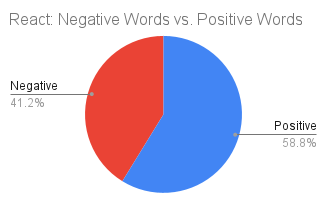
\includegraphics[scale=0.5]{react-words}    
\end{center}

In this chart we can see that react has more positive (162,415) words that represent 58.8\% compared to the negative (113,892) words, which represent 41.2\%.

\begin{center}
    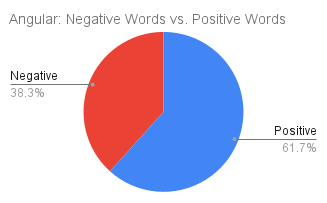
\includegraphics[scale=0.50]{angular-words}    
\end{center}

In the case of angular we have a more positive community than react with 280,779 positive words, which represents 61.7\%, compare with the 174,500 negative words which represent 38.3\%.

\begin{center}
    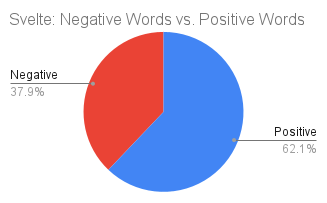
\includegraphics[scale=0.50]{svelte-words}    
\end{center}

Next, we have svelte with 35,965 positive words that represent 62.1\% and 21,948 negative words that represent 37.9\%.

\begin{center}
    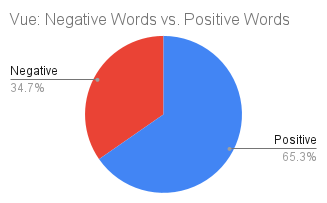
\includegraphics[scale=0.50]{vue-words}    
\end{center}

Vue has a total of 44,901 positive words, 65.3\%, and 23,821 negative words, 34.7\%.

This informations suggest that all the communities are positive in general, and there are big differences between each other, now we are going to display what are the most used words, top 20, using cloud words and for each project we are going to see if it gives us an indication of what the community looks like.

\begin{center}
    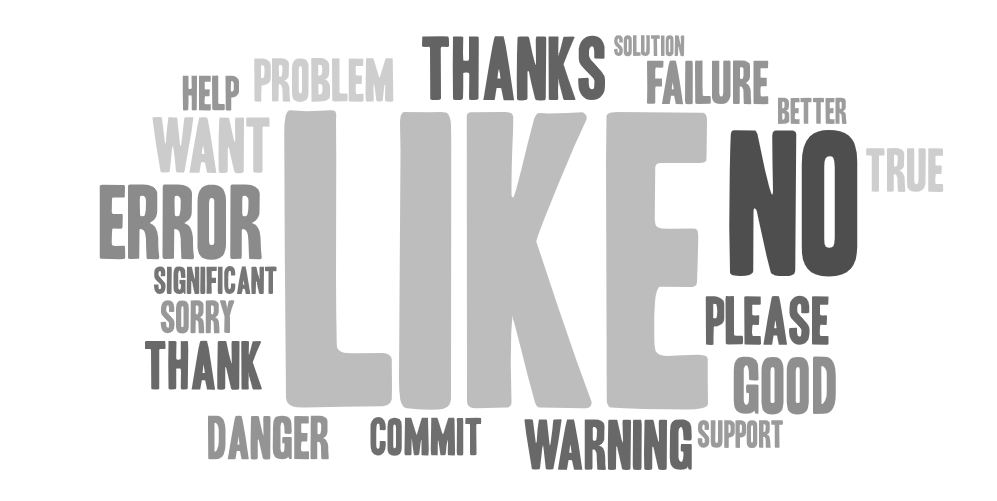
\includegraphics[scale=0.20]{react-word-cloud}    
    \textit{React}
\end{center}


\begin{center}
    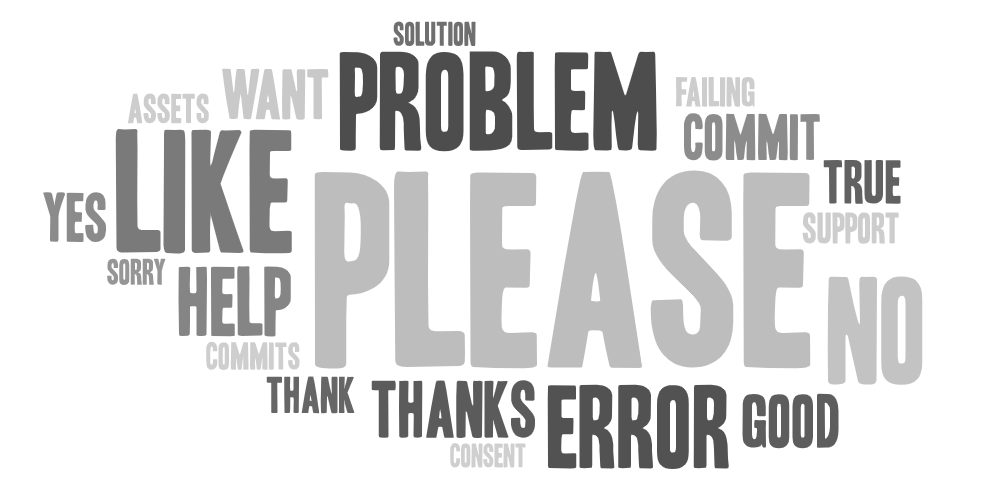
\includegraphics[scale=0.20]{angular-word-cloud}    
    \textit{Angular}
\end{center}


\begin{center}
    
\includegraphics[scale=0.20]{vue-word-cloud}    
    \textit{Vue}
\end{center}

\begin{center}
    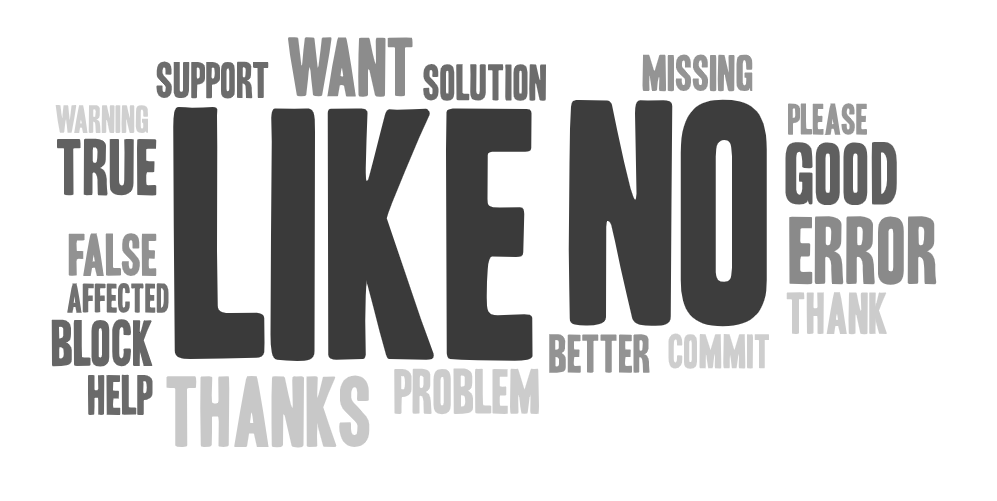
\includegraphics[scale=0.20]{svelte-word-cloud}    
    \textit{Svelte}
\end{center}

From the cloud words we can see that the most use words is \textbf{Like} and \textbf{Please}, and most uses get used accross multiple projects like \textbf{thanks}, \textbf{thank}, \textbf{good}, \textbf{no}, \textbf{problem}, which suggest that there is not a specific words that difference one community from another and overall all the communities are positive, because if we take a look at the negative words are words like \textbf{no}, \textbf{danger} or \textbf{problem} which could for fixing a particular problem.

\section{Analysis}
Compare to svelte and Vue, \textbf{react} and \textbf{angular} has received the biggest contribution overall because they were the first one while also being backed by big companies React (Facebook) and Angular (Google), which drove early adoption.

In general, all the projects have an active community and the projects are being developed, and the community seems to use the same kind of word, so there isn't any bad choice from a community side.

If we are talking about impact, if you would like to have the highest impact we would suggest Vue because they have the lowest amount of contributors which means that it's easier to leave a mark in the project, but if you want to learn new skills and have a bigger community we would suggest Angular and React, which has the largest pool of contributors.

If the contributor would like to learn something new and a different approach than the other frameworks then we would suggest Svelte, but overall the fourth project is great for the metrics that we establish, the "liveliness" and their communities

\section{Future Work}
This paper was focused mainly on the top four front-end frameworks but the approach for the community could be expanded by using more social platforms that revolve around the projects, like Reddit or StackOverflow.

Since this one is primarily social it could give us a view of how the community interacts outside of the scope of the project, while having the usage of the project as the main topic.

The approach used during this paper could be expanded for different types of projects and libraries and try to see how their community looks like, not limiting to a first-time contributor but perhaps a seasoned contributor who would like to contribute to a project on a particular area and it has multiple projects to choose from.s

